\chapter{Quản lý dự án bằng Jira}

\section{Giới thiệu}

Trong quá trình phát triển hệ thống ChatBot hỗ trợ học tập, nhóm sử dụng Jira để quản lý toàn bộ tiến độ thực hiện dự án. Jira giúp phân chia công việc cho từng thành viên, theo dõi trạng thái công việc, lập kế hoạch Sprint và đánh giá tiến độ của dự án theo từng giai đoạn.

Thông qua Jira, toàn bộ yêu cầu chức năng được chuyển thành các User Story và Task cụ thể, từ đó giúp nhóm dễ dàng phối hợp và giảm thiểu việc bỏ sót yêu cầu.

\section{Quy trình quản lý}

Nhóm áp dụng quy trình Agile Scrum với các bước:

\begin{enumerate}
	\item Phân tích yêu cầu.
	\item Tạo Epic.
	\item Chia thành các User Story.
	\item Chia nhỏ thành các Task.
	\item Thực hiện Sprint.
	\item Kiểm thử.
	\item Review và hoàn thành Sprint.
\end{enumerate}

\section{Danh sách Epic}

Các Epic chính của dự án bao gồm:

\begin{itemize}
	\item Xây dựng Backend FastAPI
	\item Xây dựng Frontend React
	\item Xây dựng Pipeline RAG
	\item Tích hợp ChromaDB
	\item Đánh giá mô hình (Benchmark)
	\item Thiết kế giao diện
	\item Kiểm thử hệ thống
	\item Viết tài liệu báo cáo
\end{itemize}
\section{User Story}

Một số User Story tiêu biểu:

\begin{itemize}
	\item Sinh viên có thể tải tài liệu môn học.
	\item Sinh viên có thể đặt câu hỏi để Chatbot tư vấn.
	\item Hệ thống trả lời thông minh dựa trên kỹ thuật RAG.
	\item Sinh viên có thể thử nghiệm thay đổi cấu hình RAG.
	\item Quản trị viên quản lý kho tài liệu trung tâm.
	\item Quản trị viên xem báo cáo hoạt động.
	\item Quản trị viên theo dõi kết quả chạy Benchmark của các mô hình.
\end{itemize}
\section{Quản lý Backlog}

\begin{figure}[H]
	\centering
	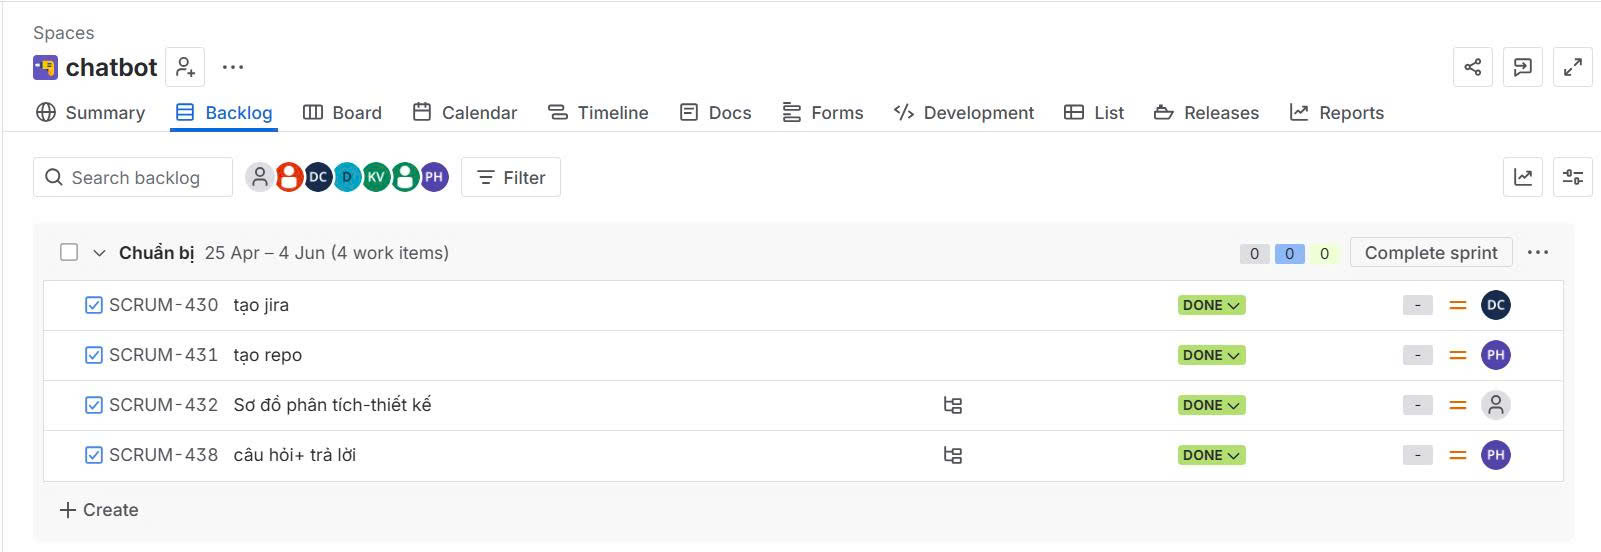
\includegraphics[width=\textwidth]{images/backlog_1}
	\caption{Product Backlog (Phần 1)}
\end{figure}

\begin{figure}[H]
	\centering
	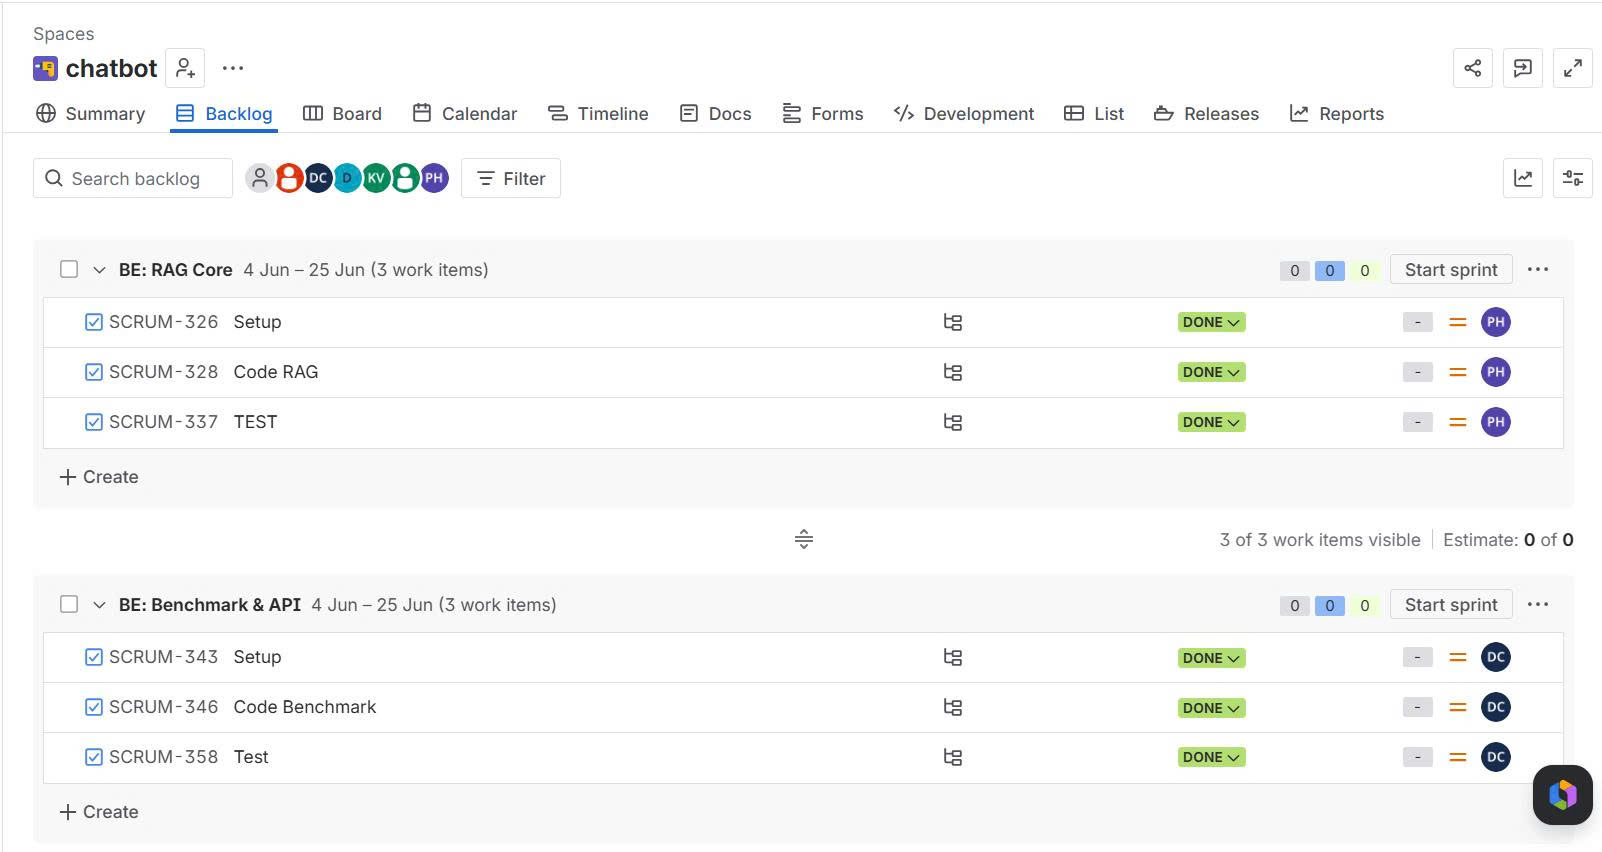
\includegraphics[width=\textwidth]{images/backlog_2}
	\caption{Product Backlog (Phần 2)}
\end{figure}

\begin{figure}[H]
	\centering
	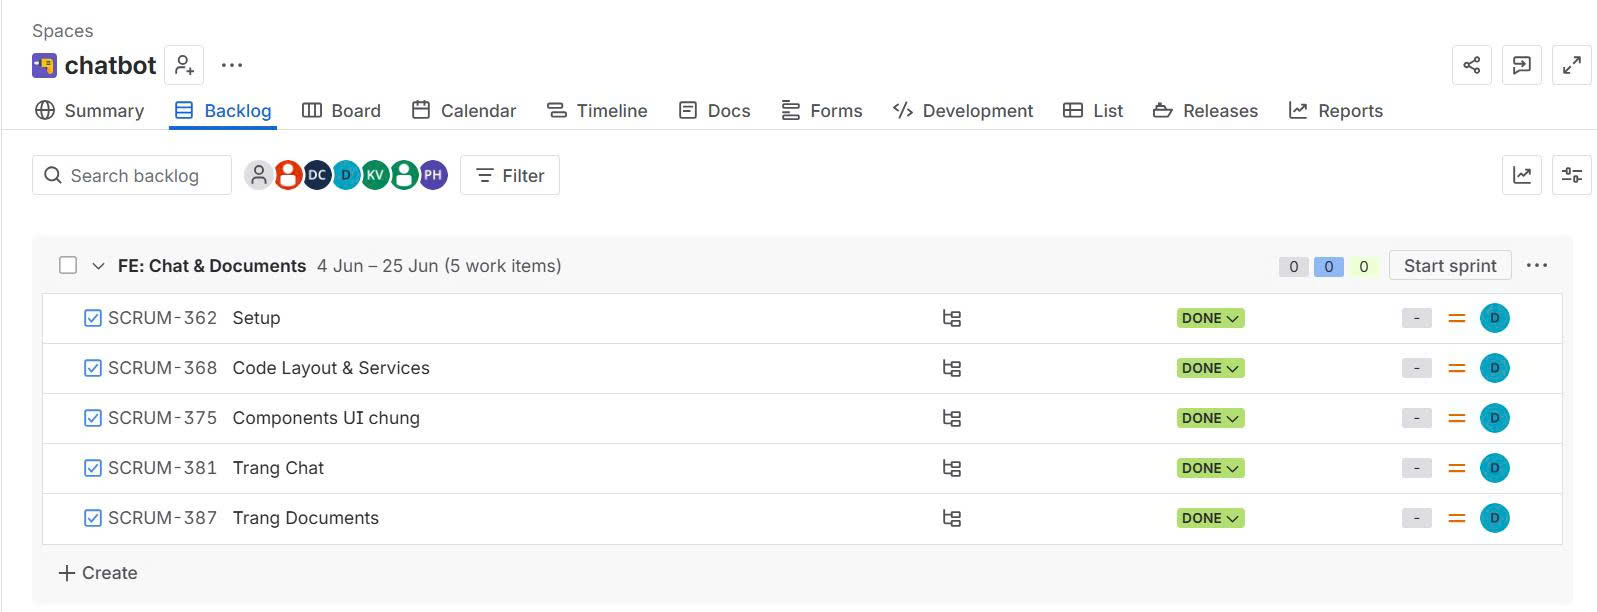
\includegraphics[width=\textwidth]{images/backlog_3}
	\caption{Product Backlog (Phần 3)}
\end{figure}

\begin{figure}[H]
	\centering
	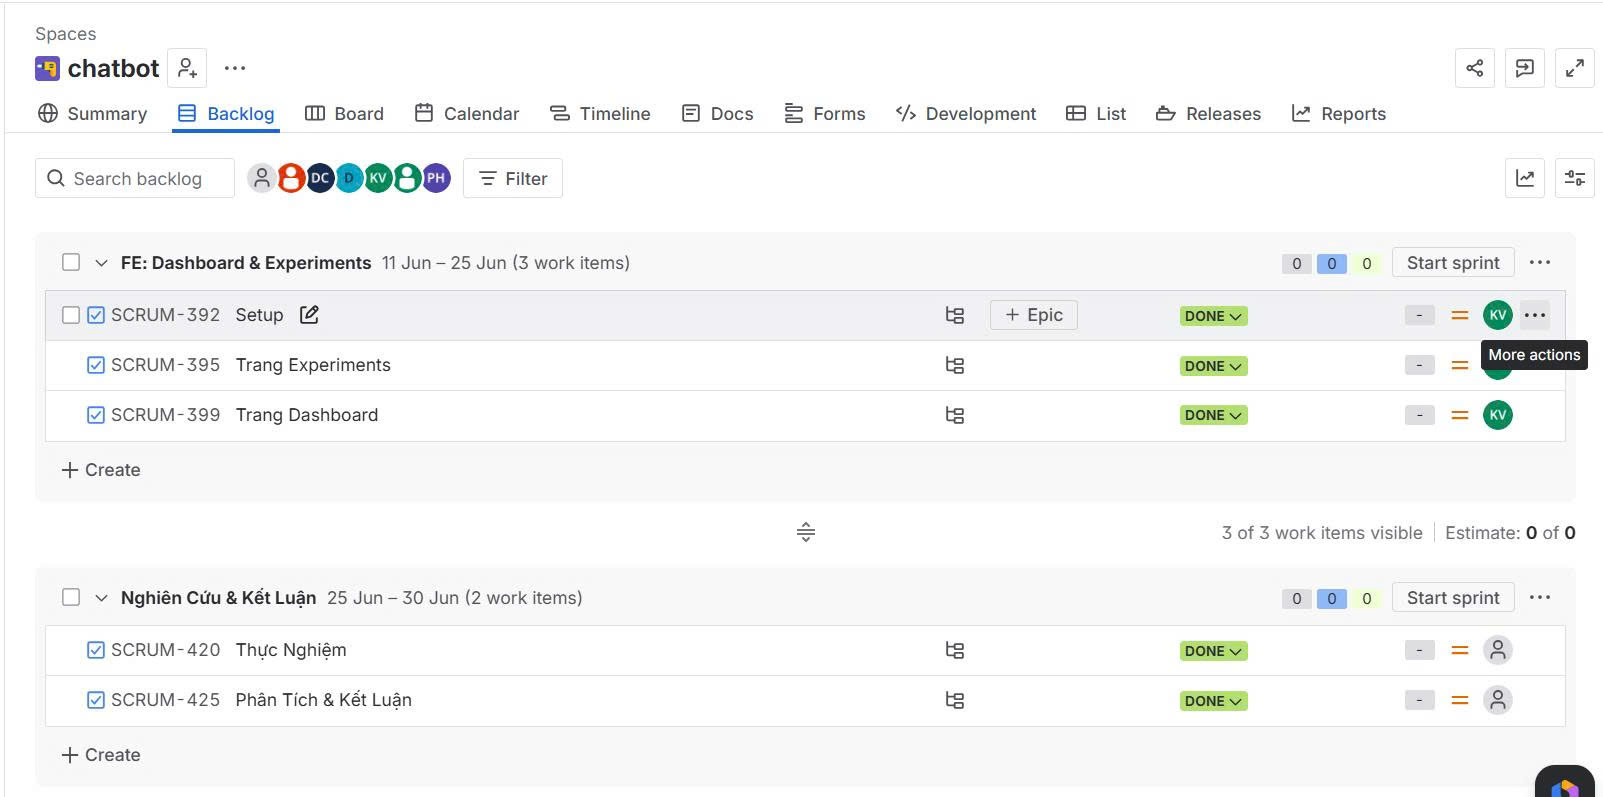
\includegraphics[width=\textwidth]{images/backlog_4}
	\caption{Product Backlog (Phần 4)}
\end{figure}

\begin{figure}[H]
	\centering
	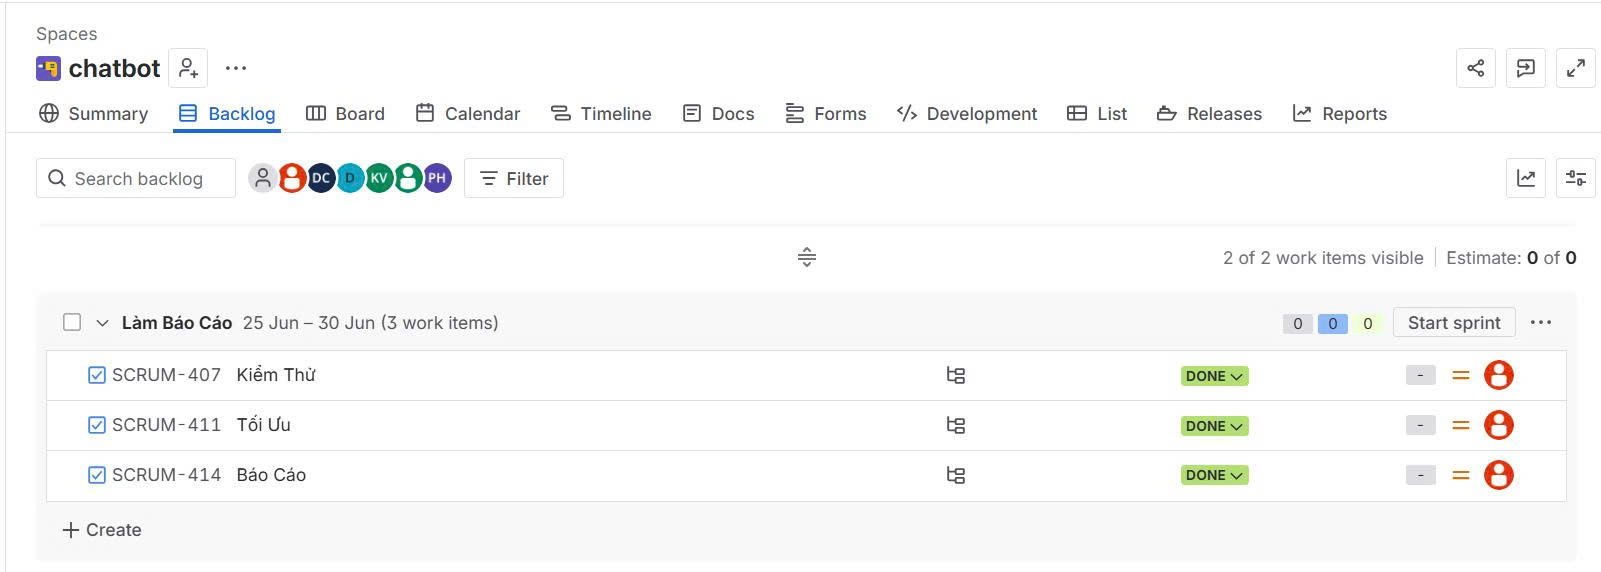
\includegraphics[width=\textwidth]{images/backlog_5}
	\caption{Product Backlog (Phần 5)}
\end{figure}
\section{Kế hoạch Sprint}

Dự án được chia thành nhiều Sprint.

\begin{table}[H]
	\centering
	\begin{tabular}{|c|p{6cm}|c|}
		\hline
		Sprint & Nội dung & Trạng thái\\
		\hline
		Sprint 1 & Thiết kế kiến trúc hệ thống & Hoàn thành\\
		\hline
		Sprint 2 & Xây dựng Backend FastAPI & Hoàn thành\\
		\hline
		Sprint 3 & Xây dựng Frontend React & Hoàn thành\\
		\hline
		Sprint 4 & Tích hợp ChromaDB và RAG & Hoàn thành\\
		\hline
		Sprint 5 & Cấu hình và thử nghiệm Benchmark & Hoàn thành\\
		\hline
		Sprint 6 & Benchmark và đánh giá & Hoàn thành\\
		\hline
		Sprint 7 & Kiểm thử và sửa lỗi & Hoàn thành\\
		\hline
		Sprint 8 & Hoàn thiện báo cáo & Hoàn thành\\
		\hline
	\end{tabular}
	\caption{Kế hoạch Sprint của dự án}
\end{table}
\section{Quy trình xử lý công việc}

Mỗi công việc trên Jira đều trải qua các trạng thái:

\begin{center}
	Backlog
	$\rightarrow$
	To Do
	$\rightarrow$
	In Progress
	$\rightarrow$
	Code Review
	$\rightarrow$
	Testing
	$\rightarrow$
	Done
\end{center}

Việc chuẩn hóa quy trình giúp nhóm dễ dàng theo dõi tiến độ và biết được chính xác công việc đang ở giai đoạn nào.

\section{Quản lý công việc trên Jira}

\begin{figure}[H]
	\centering
	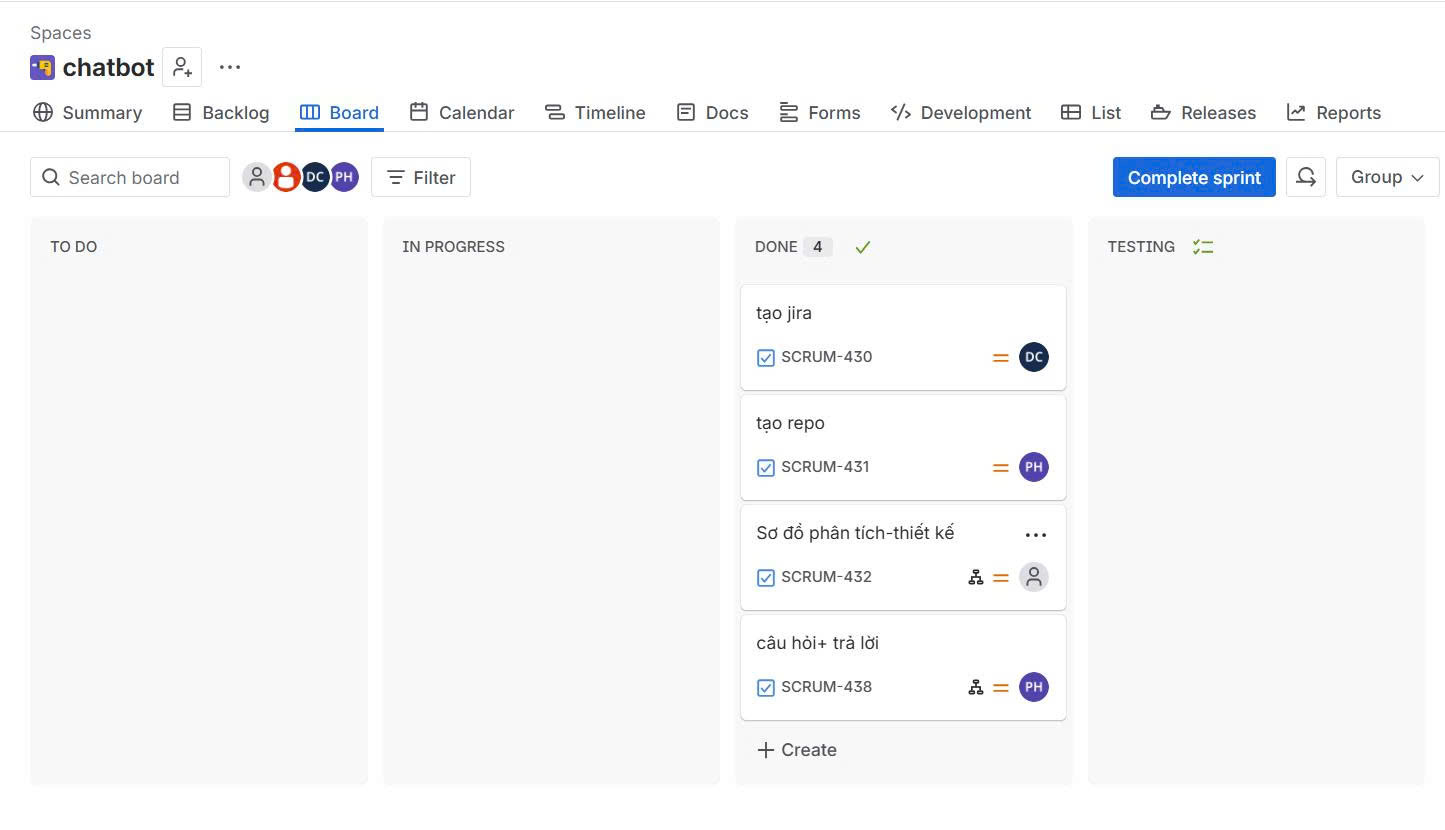
\includegraphics[width=\textwidth]{images/jira_board.png}
	\caption{Bảng Kanban quản lý công việc trên Jira}
	\label{fig:jira_board}
\end{figure}
Hình trên thể hiện toàn bộ bảng Kanban của dự án. Mỗi thẻ đại diện cho một nhiệm vụ cụ thể và được di chuyển giữa các cột Backlog, To Do, In Progress, Testing và Done trong suốt vòng đời phát triển phần mềm.

\section{Phân công công việc}

\begin{table}[H]
	\centering
	\begin{tabular}{|p{5cm}|p{5cm}|}
		\hline
		Công việc & Thành viên\\
		\hline
		Thiết kế hệ thống &...\\
		Backend FastAPI & ...\\
		Frontend React & ...\\
		RAG Pipeline & ...\\
		Đánh giá Benchmark &...\\
		Kiểm thử & ...\\
		Viết tài liệu & ...\\
		\hline
	\end{tabular}
	\caption{Phân công công việc}
\end{table}
\section{Đánh giá}

Việc sử dụng Jira mang lại nhiều lợi ích trong quá trình phát triển dự án:

\begin{itemize}
	\item Theo dõi tiến độ theo thời gian thực.
	\item Phân chia công việc rõ ràng.
	\item Hỗ trợ lập kế hoạch Sprint.
	\item Quản lý lịch sử thay đổi.
	\item Hỗ trợ báo cáo tiến độ cho giảng viên.
	\item Dễ dàng phối hợp giữa các thành viên.
\end{itemize}

Nhờ Jira, nhóm quản lý tốt tiến độ thực hiện, giảm thiểu việc chồng chéo công việc và đảm bảo hoàn thành dự án đúng thời hạn.

\chapter{Quản lý Repository trên GitHub}

Trong quá trình phát triển, nhóm sử dụng GitHub làm nền tảng lưu trữ và quản lý mã nguồn. Repository là nơi tập trung toàn bộ mã nguồn của dự án, bao gồm Backend, Frontend, tài liệu thiết kế và các tệp cấu hình. Việc sử dụng GitHub giúp các thành viên dễ dàng cộng tác, theo dõi lịch sử thay đổi và đồng bộ công việc.

\begin{figure}[H]
	\centering
	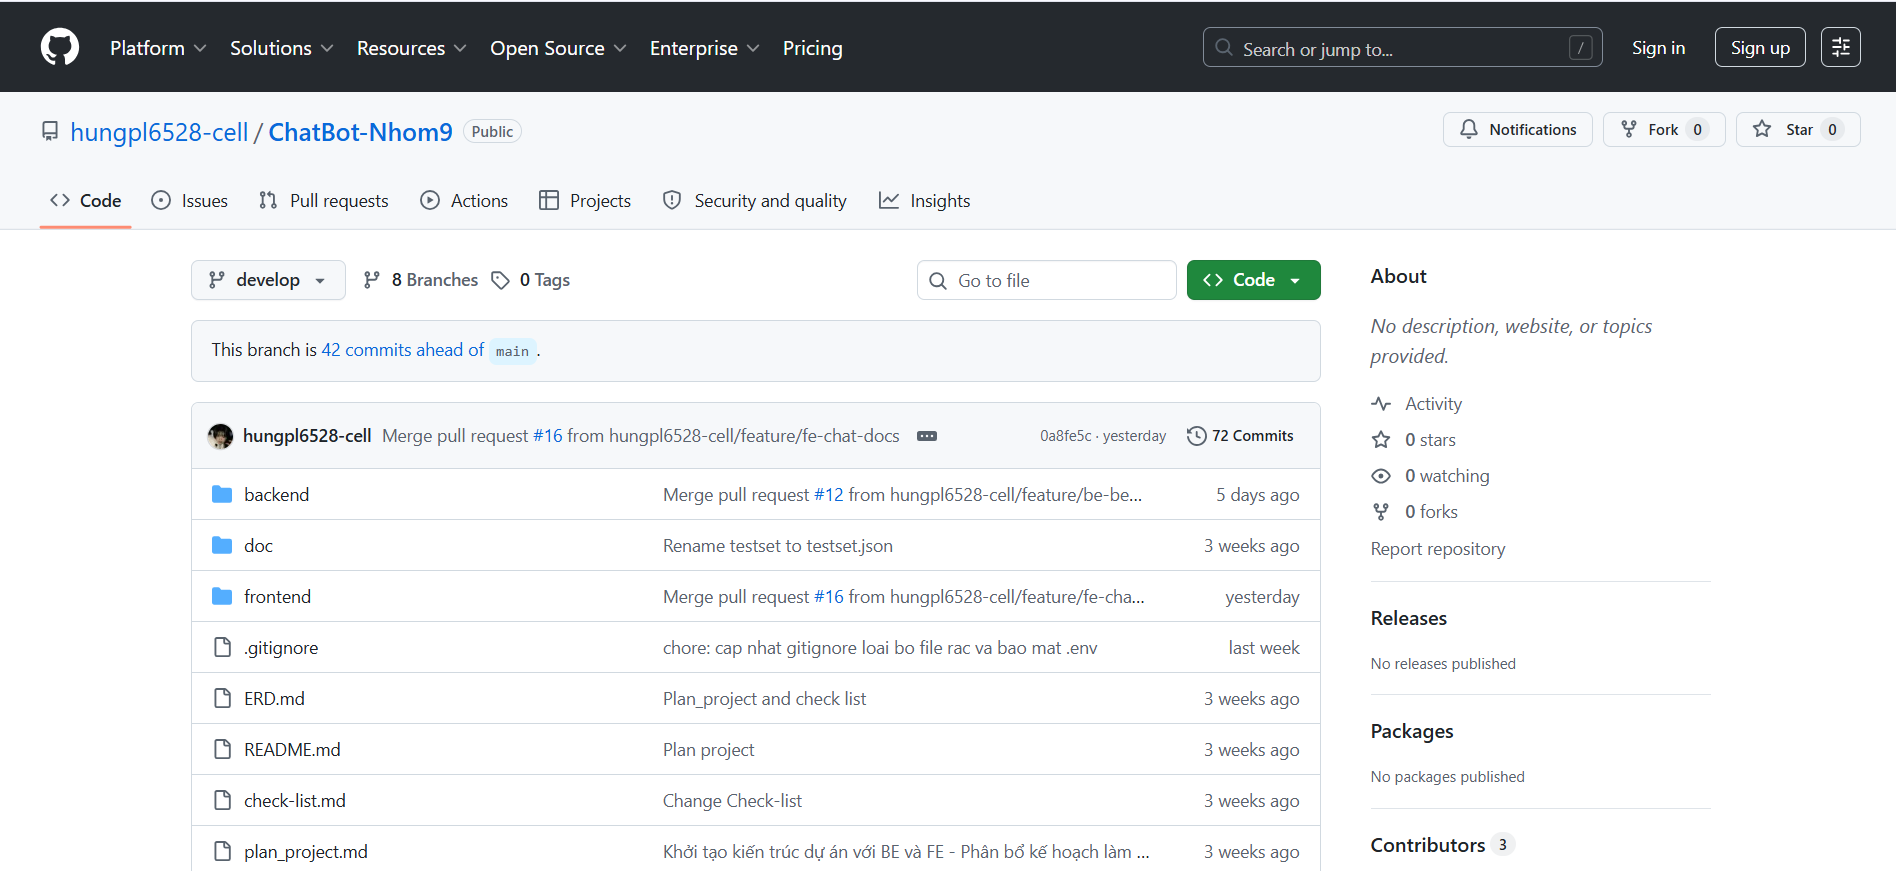
\includegraphics[width=\textwidth]{images/github_repository}
	\caption{Repository của dự án trên GitHub}
	\label{fig:github_repository}
\end{figure}

Hình trên cho thấy kho mã nguồn của dự án được quản lý trên GitHub. Repository bao gồm các thư mục chính như \texttt{backend}, \texttt{frontend} và \texttt{doc}. Ngoài ra, nhóm sử dụng nhiều nhánh (Branch) để phát triển song song các chức năng, kết hợp với Pull Request nhằm kiểm tra mã nguồn trước khi hợp nhất vào nhánh chính.

\subsection{Cấu trúc dự án}

\begin{figure}[H]
	\centering
	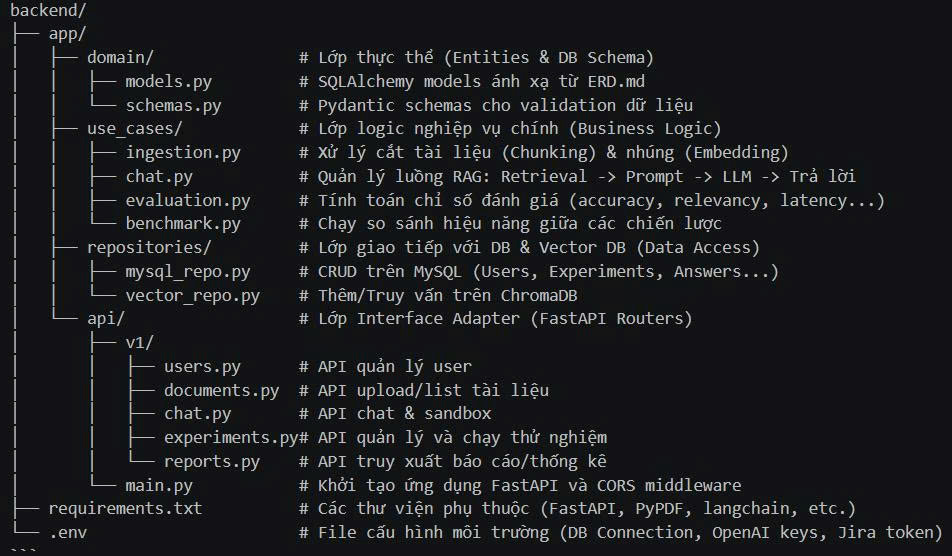
\includegraphics[width=0.95\textwidth]{images/project_structure}
	\caption{Cấu trúc thư mục Backend của hệ thống}
	\label{fig:project_structure}
\end{figure}
\subsection{Lịch sử Commit}

Trong quá trình phát triển, nhóm sử dụng Git để ghi nhận toàn bộ lịch sử thay đổi của mã nguồn. Mỗi chức năng sau khi hoàn thành đều được Commit với nội dung mô tả rõ ràng trước khi được Push lên GitHub. Việc này giúp các thành viên dễ dàng theo dõi tiến độ, kiểm tra lịch sử thay đổi, khôi phục phiên bản khi cần thiết và hỗ trợ làm việc nhóm hiệu quả.

\begin{figure}[H]
	\centering
	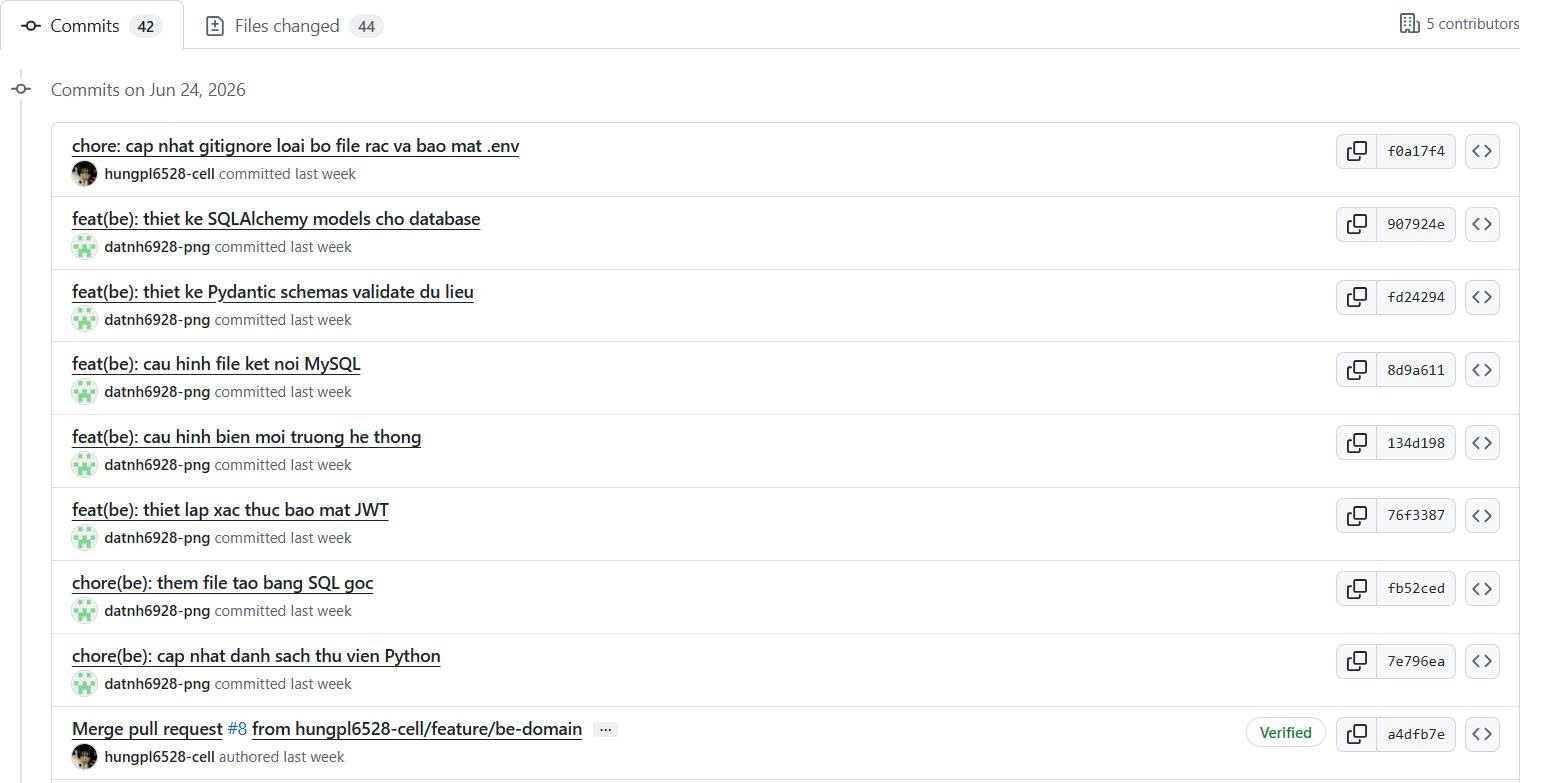
\includegraphics[width=\textwidth]{images/github_commit1}
	\caption{Lịch sử Commit của dự án trên GitHub}
	\label{fig:github_commit1}
\end{figure}

Hình trên thể hiện lịch sử Commit của dự án trong suốt quá trình phát triển. Mỗi Commit tương ứng với một lần cập nhật hoặc bổ sung chức năng mới cho hệ thống. Nội dung Commit được mô tả ngắn gọn nhằm phản ánh chính xác thay đổi của mã nguồn.
\begin{figure}[H]
	\centering
	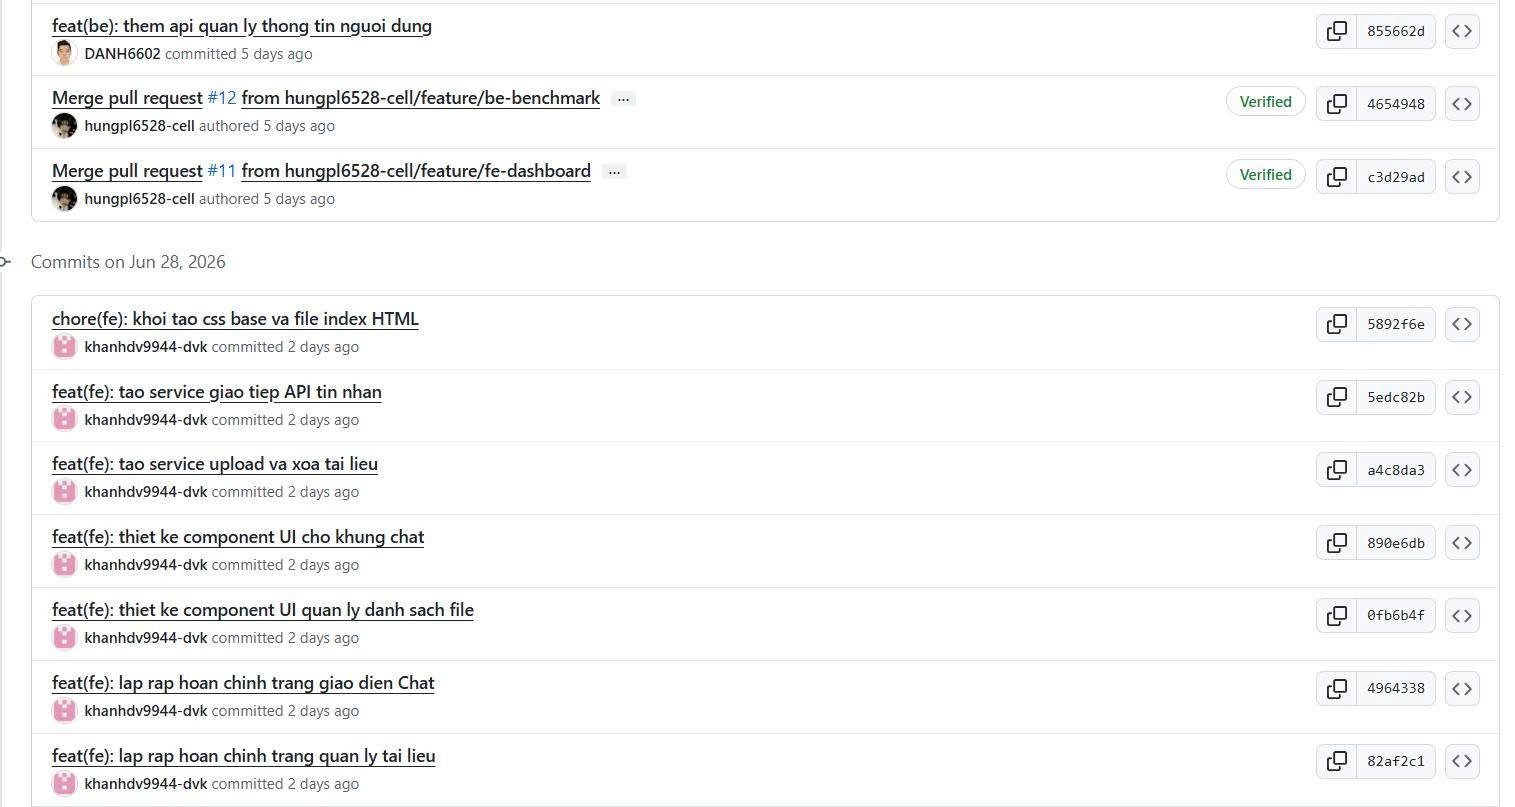
\includegraphics[width=\textwidth]{images/github_commit2}
	\caption{Lịch sử Commit (tiếp theo)}
	\label{fig:github_commit2}
\end{figure}

\begin{figure}[H]
	\centering
	\caption{Lịch sử Commit (tiếp theo)}
	\label{fig:github_commit3}
\end{figure}
Việc sử dụng Git và GitHub giúp nhóm:

\begin{itemize}
	\item Quản lý phiên bản mã nguồn.
	\item Theo dõi lịch sử thay đổi.
	\item Hỗ trợ làm việc nhóm.
	\item Hạn chế xung đột mã nguồn.
	\item Dễ dàng khôi phục các phiên bản trước.
	\item Tích hợp chặt chẽ với Jira thông qua Issue và Commit.
\end{itemize}


